\section{Motivation}
Coverage is necessary for a rapid-response Earth-observation mission, but it is not sufficient. A satellite can pass over a target within minutes and still miss the opportunity if the task arrives after the pass. The opposite can also happen: a request can spread through the network while no informed satellite obtains a useful access before the deadline. This thesis therefore treats information delivery and orbital access as two connected stages of one operational problem.

Wildfire monitoring provides a concrete case. A source product first has to become a request with a position, release time, priority, deadline, and message size. That request must then move through intermittent ground-to-space and space-to-space contacts. Only after reception can a satellite use a later access for follow-up observation. Figure~\ref{fig:mission_chain} shows this sequence and the two principal failure modes.

\begin{figure}[htbp]
\centering
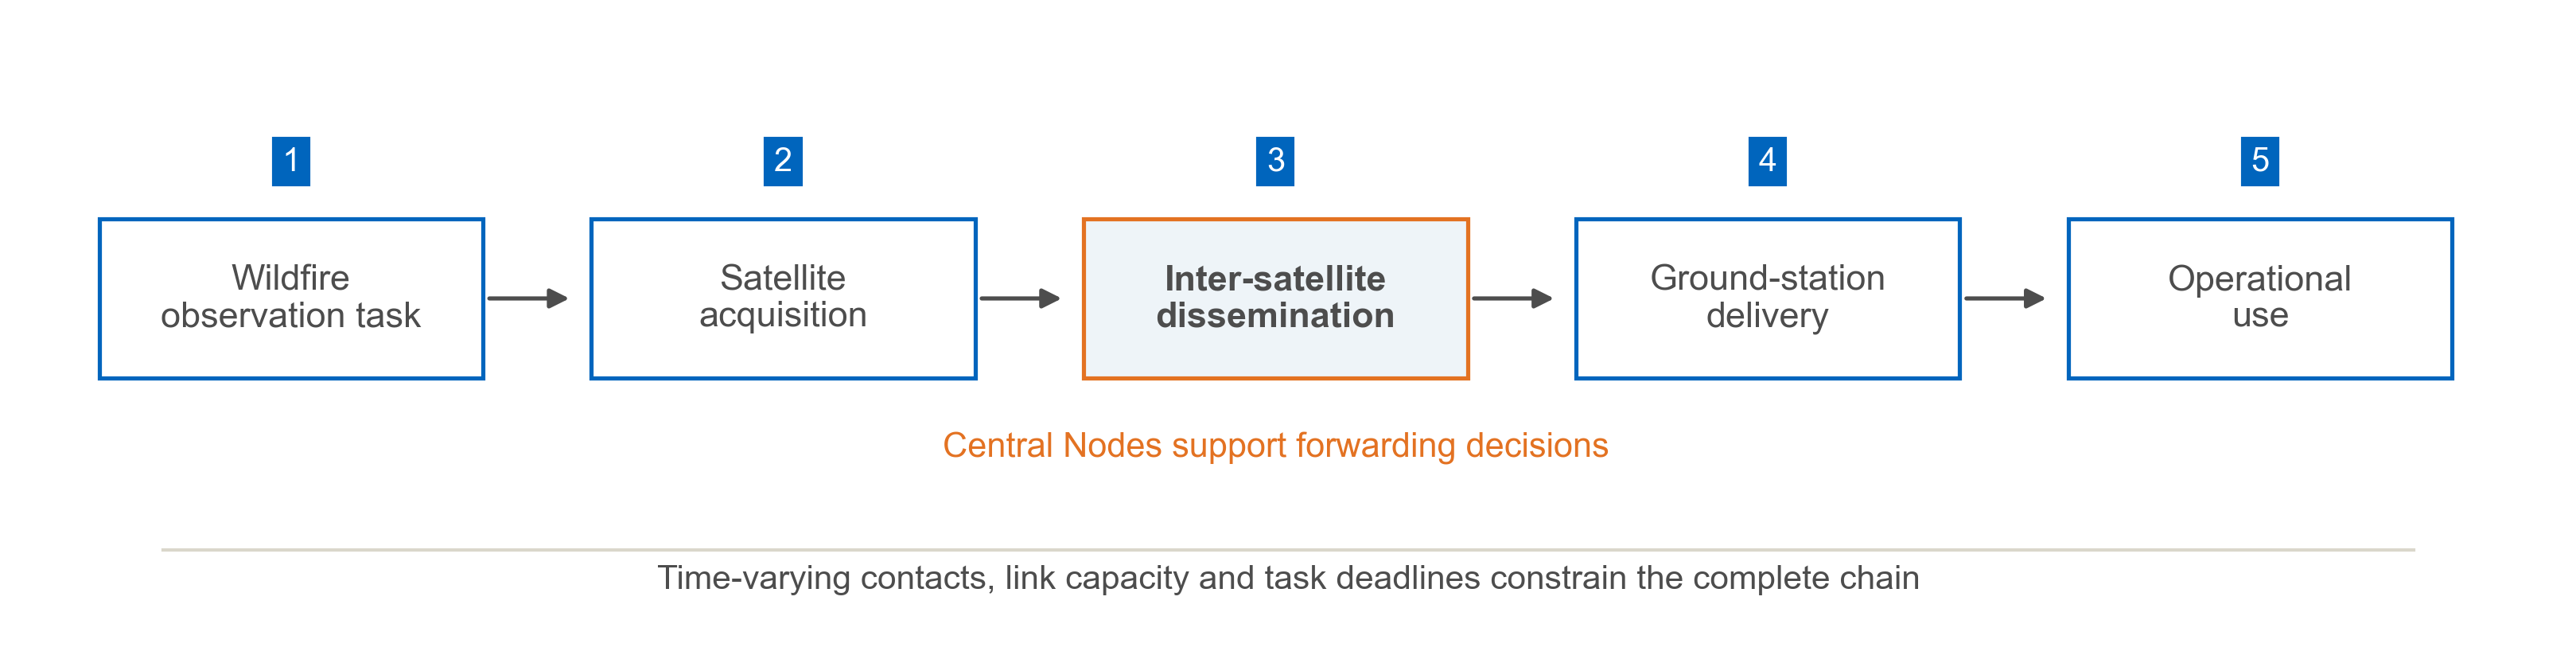
\includegraphics[width=0.96\textwidth]{figures/part1_revision/mission_chain.png}
\caption{Operational chain used in the thesis. Communication and geometry are separate requirements, and observation is credited only after complete task reception.}
\label{fig:mission_chain}
\end{figure}
A central node is a satellite assigned additional routing capabilities. In this study it acts as a preferred relay: the label changes which links may be used, how forwarding candidates are ordered, and the assumed communication range for links involving that node. It does not make all constellation decisions and it does not receive a different orbit, sensor, processor, or reliability model. This definition follows the role of collaborative information brokers in federated satellite systems \citep{Scrocciolani2024,Messina2025} while keeping observation authority distributed.

The design question is not simply whether central nodes help. Too few may leave gaps in the temporal communication graph. Too many may add unnecessary differentiated spacecraft, duplicate traffic, or concentrate operation around one routing mechanism. The useful fraction can also change with constellation geometry, workload, packet size, and routing constraints. The thesis therefore evaluates the full trade-space instead of selecting a central-node fraction from a single performance metric.

\section{Problem Statement}
The starting point was an existing communication and TAT-C-based orbital model supplied by Vincenzo Messina. This thesis adapts that basis to time-stamped wildfire follow-up tasks and makes task reception a condition for observation credit. The adapted problem contains many tasks released at different times, four priority classes, finite packets, different deadlines, and two event windows with very different loads.

The engineering problem is:

Determine how Walker-constellation geometry, routing policy, and the fraction of central nodes affect deadline-constrained task dissemination and post-reception wildfire observation, while retaining the communication burden and response to failures needed for an architecture decision.

Two uses of the word robustness are separated throughout the report. Physical robustness is the retained mission performance after a node, link, ground-station, or capacity disturbance. Decision stability is the persistence of an architecture ranking when the objective weights change. A design can be stable under a weighting model and still perform poorly after a physical failure.

\section{Aim and Objectives}
The aim is to construct a traceable performance-resource-robustness trade-space for communication-constrained wildfire follow-up in a distributed satellite system. Four objectives support that aim:

\begin{enumerate}
\item Convert Sentinel-3 active-fire detections into a reproducible task table with location, release time, priority, deadline, packet size, and source provenance.
\item Simulate reception, finite-capacity forwarding, and post-reception observation over a controlled Walker-constellation and central-node design grid.
\item Compare mission performance, communication burden, and failure response without treating one metric or an unadjusted correlation as a complete architecture decision.
\item Identify Pareto-efficient and decision-stable candidates while stating the assumptions under which the shortlist is valid.
\end{enumerate}
The objectives deliberately separate data preparation, simulation, and decision support. This prevents the architecture comparison from changing silently when the task definition or the ranking preference changes.

\section{Research Questions}
The report answers three research questions:

\textbf{RQ1.} How do central-node fraction and forwarding policy change timely task dissemination and follow-up observation in the implemented distributed satellite system?

\textbf{RQ2.} How do workload, packet size, constellation geometry, and injected failures change performance and the relative ranking of architectures?

\textbf{RQ3.} Which architectures provide defensible trade-offs among observation fulfilment, deadline-complete dissemination, communication burden, resource proxies, and robustness?

These questions replace the earlier five-question structure. Task generation is treated as the input method that enables the experiment, not as a separate research question. Observation-radius, placement, and central-node component ablations remain validity checks and future work unless the corresponding runs are available.

\section{Expected Relationships}
The literature and the temporal-network model motivate three expectations rather than five stand-alone hypotheses. First, adding initial relay capability should create useful temporal paths, but the marginal benefit should decrease once most relevant paths already exist \citep{Burleigh2022,Araniti2015,CCSDS2019}. Second, faster or broader dissemination can require more transfers and differentiated nodes, so minimum delay alone should not identify the preferred architecture. Third, the preferred design should depend on workload and preference assumptions because communication capacity, deadlines, and resource burden compete. These expectations organize the analysis; they are not treated as results before the simulation is evaluated.

\section{Scope and Boundaries}
The simulated mission begins when a processed wildfire task is released. It ends when the report has evaluated task reception and a possible follow-up observation. Thermal measurement, onboard fire detection, cloud screening, image production, image downlink, and delivery of an alert to civil-protection authorities are outside the model.

The central-node fraction is the primary treatment. Satellite count, plane count, altitude, and inclination form the architecture context. Packet-size multipliers, routing policy, node and link failures, ground-station outage, capacity degradation, and objective weights are tested sensitivities. The following assumptions remain fixed in the completed campaign:

\begin{itemize}
\item one deterministic balanced central-node placement rule;
\item one bundled central-node treatment combining eligibility, preference, and a link-budget multiplier;
\item a 700 km observation-radius proxy;
\item one Munich ground station in the baseline;
\item two selected event windows rather than a statistical sample of global fire conditions; and
\item engineering resource proxies rather than monetary lifecycle cost.
\end{itemize}
The 60- and 120-satellite regional comparison uses the intended 32-task California and 773-task India inputs. The completed 180-satellite India layer used a consistent 741-task population because of an index-alignment error in task normalization. It remains useful for within-population sensitivity, but it is not pooled with the matched regional comparison or used to claim a clean 120-to-180 scaling law. This provenance issue is explained with the validation procedure in Section 4.8 rather than on a separate front-matter page.

\section{Contributions}
The thesis makes three connected contributions.

\begin{enumerate}
\item \textbf{A traceable wildfire-task input.} The final table links Sentinel-3 product records to de-duplicated fire-region tasks and preserves the information needed to reproduce their priority and deadline assignments.
\item \textbf{A communication-aware architecture experiment.} The model separates physical opportunities, accepted transfers, task reception, and observation. It evaluates the same task rows across a full Walker and central-node grid, with finite capacity and deterministic replay.
\item \textbf{A robustness-aware decision method.} Raw metrics are validated before Pareto filtering. Failure response and objective-weight sensitivity are reported separately, so the final shortlist remains conditional and auditable.
\end{enumerate}
Vincenzo Messina supplied the original communication-model and TAT-C basis. The work developed in this thesis covers wildfire-task processing, simulator integration, central-node placement, campaign execution and resume controls, validation, post-processing, statistical analysis, figures, and report synthesis.

\section{Report Structure}
Chapter 2 connects distributed satellite coordination, temporal routing, and active-fire sensing, then states the research gap. Chapter 3 explains how Sentinel-3 detections become the fixed task input. Chapter 4 presents the system model and simulation sequence. The later part of the thesis defines the experimental contract, reports nominal and Fresh V2 results, performs sensitivity and robustness analysis, and turns the validated metrics into a conditional architecture shortlist. Detailed software operation, file formats, and checkpointing belong in the appendices and repository documentation rather than in the core methodology narrative.
